% SEE GITHUB REPO AT https://github.com/gboeing/gis-bok-notebooks

\RequirePackage[l2tabu,orthodox]{nag}
\documentclass[11pt,letterpaper]{article}
\usepackage[T1]{fontenc}
\usepackage[utf8]{inputenc}
\usepackage{crimson}
\usepackage{helvet}
\usepackage[strict,autostyle]{csquotes}
\usepackage[USenglish]{babel}
\usepackage{microtype}
\usepackage{authblk}
\usepackage{booktabs}
\usepackage{caption}
\usepackage{endnotes}
\usepackage{geometry}
\usepackage{graphicx}
\usepackage{hyperref}
\usepackage{natbib}
\usepackage{rotating}
\usepackage{setspace}
\usepackage{titlesec}
\usepackage{url}
\usepackage{color, soul}

% location of figure files, via graphicx package
\graphicspath{{./figures/}}

% configure the page layout, via geometry package
\geometry{
	paper=letterpaper,
	top=4cm,
	bottom=4cm,
	left=4cm,
	right=4cm}
\setstretch{1.02}
\clubpenalty=10000
\widowpenalty=10000

% set section/subsection headings as the sans serif font
\titleformat{\section}{\normalfont\sffamily\large\bfseries}{\thesection.}{0.3em}{}
\titleformat{\subsection}{\normalfont\sffamily\small\bfseries}{\thesubsection.}{0.3em}{}

% make figure/table captions sans-serif small font
\captionsetup{font={footnotesize,sf},labelfont=bf,labelsep=period}

% configure pdf metadata and link handling
\hypersetup{
	pdfauthor={Geoff Boeing and Daniel Arribas-Bel},
	pdftitle={GIS and Computational Notebooks},
	pdfsubject={GIS and Computational Notebooks},
	pdfkeywords={GIS,},
	pdffitwindow=true,
	breaklinks=true,
	colorlinks=false,
	pdfborder={0 0 0}}

\title{GIS and Computational Notebooks}
\author{Geoff Boeing and Dani Arribas-Bel}
\date{2020}

\begin{document}

\maketitle

\begin{abstract}
Nunc efficitur dui non elementum tincidunt. Sed eget ultricies dui, nec congue massa. Fusce at faucibus arcu, a dapibus leo. Donec congue viverra lorem, et viverra massa pellentesque eu. Mauris dictum efficitur lectus, nec tempus velit viverra at. Pellentesque habitant morbi tristique senectus et netus et malesuada fames ac turpis egestas. In tristique urna purus, a viverra sapien vehicula at. Donec id lectus dui. Class aptent taciti sociosqu ad litora torquent per conubia nostra, per inceptos himenaeos. Ut viverra leo ac velit aliquam, id pellentesque est maximus. Proin laoreet aliquet ex vel semper. Integer congue sollicitudin elit, ut tincidunt odio tincidunt quis. Duis eu mi sed massa pellentesque efficitur.
%\vspace{1cm}
\end{abstract}

\section*{Definitions}

\begin{itemize}
    \item \textbf{Computational Notebook}: a computer file containing code, output, images, and narrative text woven together.
    \item \textbf{Interactive Computing}: x
    \item \textbf{Jupyter Notebook}: an interactive computing environment comprising a web browser, a notebook server, a notebook file, and a kernel.
    \item \textbf{JupyterLab}: the notebook user interface in the Jupyter ecosystem, rendered by a web browser.
    \item \textbf{Open Science}: x
    \item \textbf{Open Source Software}: x
\end{itemize}

\section{Introduction}

A computational notebook is a computer file that contains code, output, images, and narrative text woven together. Notebooks allow users to consolidate their analytics workflow code, documentation, and results into a single reproducible and distributable package. They also enable interactive computing in the literate programming paradigm. This chapter introduces these concepts, positions computational notebooks as a key emerging tool in the GIS landscape, and discusses their value for geospatial analysts.

The notebook interface was first developed in the 1980s by Mathematica as a closed-source commercial tool for scientists \citep{somers_scientific_2018}. During the 2010s, open-source notebook development, spearheaded by Project Jupyter, expanded throughout research and practice by supporting popular languages in the open-source and open-science communities such as Python, R, and Julia. Today many geospatial scholars and practitioners use notebooks to load, clean, filter, analyze, visualize, and model spatial data, as well as to share their workflows and findings with peers.

Recent years have witnessed rapid adoption of computational notebooks, particularly Jupyter notebooks, among data scientists and instructors across disciplines like biology, astronomy, economics, and geography \citep{perkel_why_2018}. To understand this shift, we must consider notebooks' capabilities and the value they create for analysts, researchers, teachers, and students.

\section{How Computational Notebooks Work}

\subsection{The Paradigm}

Scientific researchers and analysts historically used lab notebooks to record their workflow's questions, hypotheses, data, models, results, and all the various analytical decisions made along the way. This was critical for organizing research activities and documenting all the \enquote{whats,} \enquote{whys,} and \enquote{hows} of the serpentine scientific process for subsequent recollection and replication. Computational notebooks mimic these traditional lab notebooks digitally and enhance them through two paradigms: literate programming and interactive computing.

To explain these computational paradigms, let us contrast them with a traditional computer program which consists of lines of code and optional inline comments and is executed linearly from beginning to end. In literate programming, a computer program instead consists of both code and natural language narratives woven together to explain and document the logic of the program \citep{knuth_literate_1992}. In interactive computing, a computer program interacts in real-time with its user and these interactions shape its execution flow \citep{perez_ipython:_2007}.

Thus, while a traditional program runs through its code in order line-by-line, a computational notebook can be executed nonlinearly and can include natural language narratives documenting and explaining each chunk of code alongside its results and output.

\begin{figure*}[tbp]
	\centering
	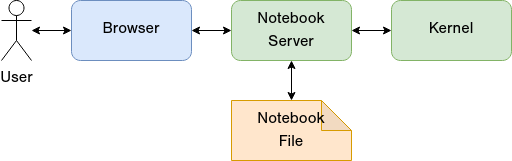
\includegraphics[width=0.8\textwidth]{notebook-architecture.png}
	\caption{Architecture of the Jupyter notebook computing environment.}
	\label{fig:notebook_architecture}
\end{figure*}

\subsection{Notebook Architecture}

Many different kinds of computational notebooks exist today for many different programming languages, but all of these various implementations share a set of common features. As the Jupyter notebook has become by far the most prominent, we will focus our discussion on it as an illustrative example.

The architecture of a Jupyter notebook comprises four components: a web browser, a notebook server, a notebook file, and a kernel \citep{kluyver_jupyter_2016}. As illustrated in Figure \ref{fig:notebook_architecture}, a user uses the web browser to browse to the notebook server, which reads the notebook file and sends it to the browser. The browser renders the notebook as a web page with individual cells in which the user can type code or text.

When the user executes a code cell, the browser sends that code to the server, which passes it to the kernel, a back-end interpreter which runs the code and returns the result to the browser via the notebook server. The browser renders this result inline in the notebook beneath the code cell. Thus, computational output such as individual calculations, tables, or figures appears beside the code that generated it.

Notebook kernels are language-specific. Hundreds of Jupyter kernels exist for dozens of different programming languages. The most popular languages for data science are all supported, including Python, R, and Julia.

\begin{figure*}[tbp]
	\centering
	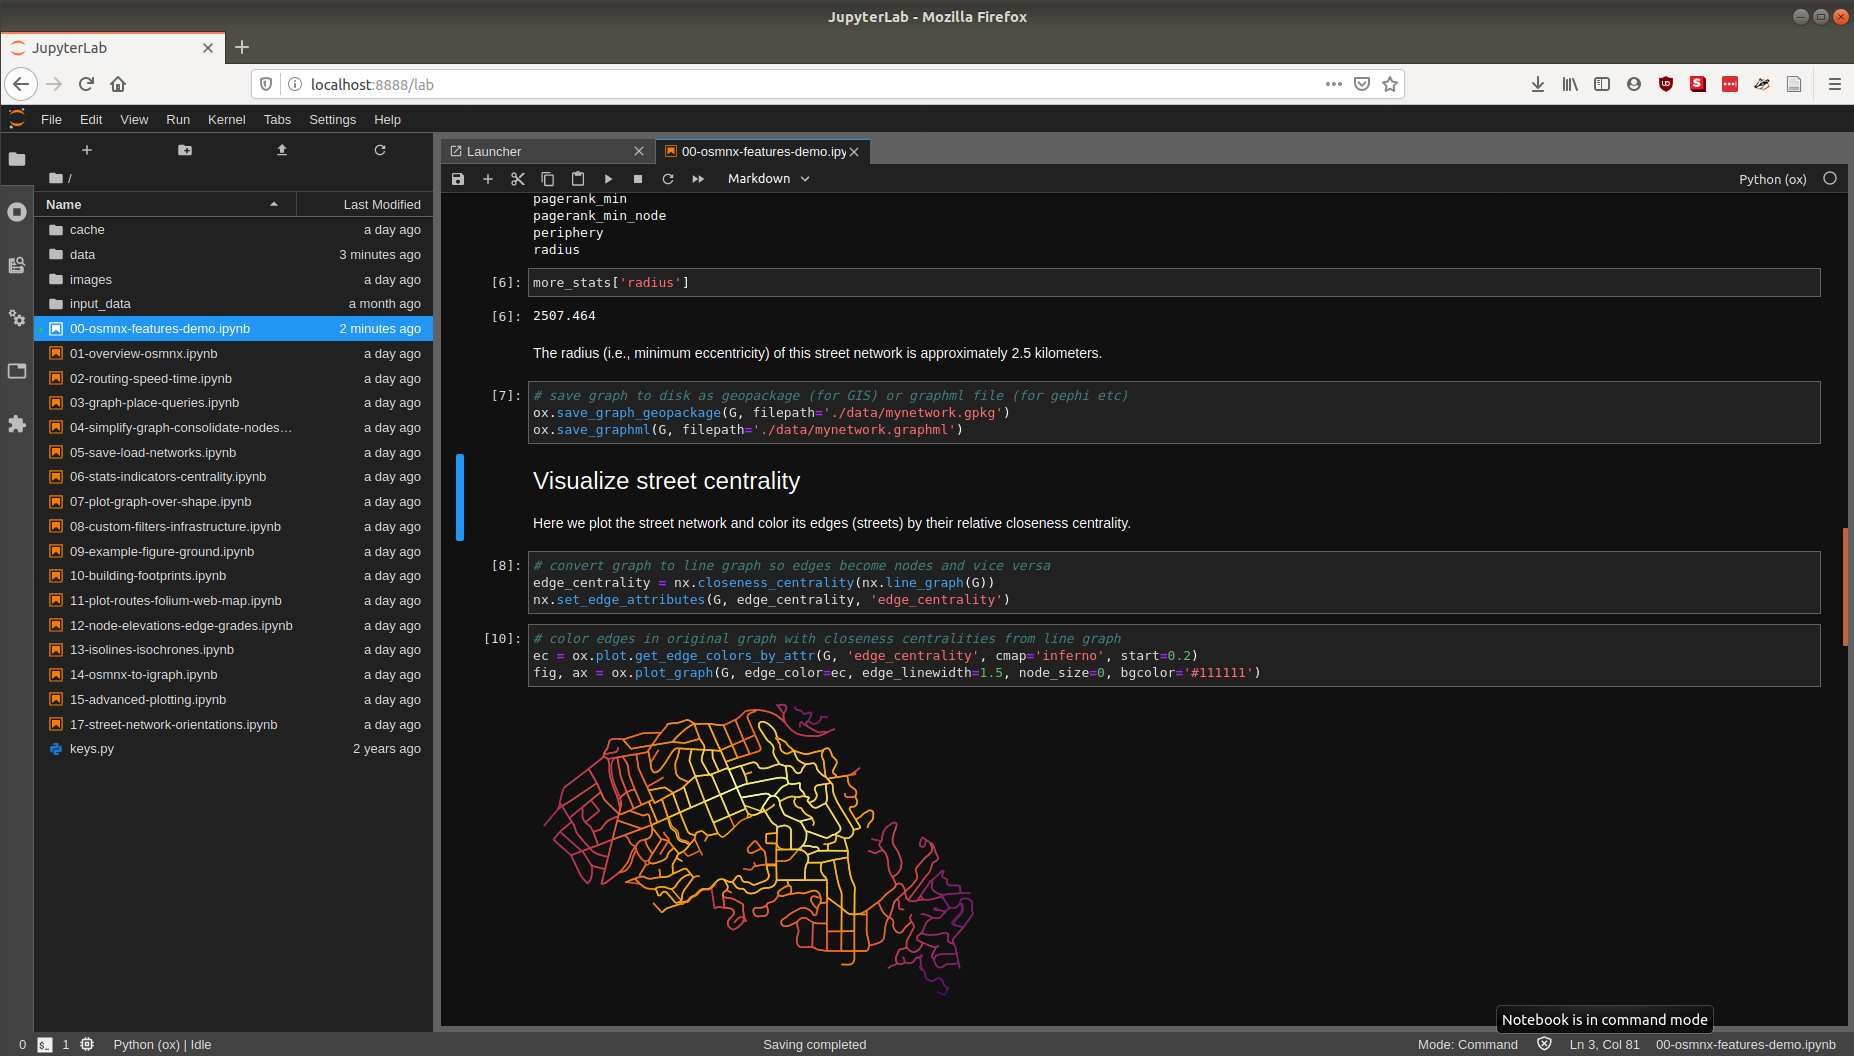
\includegraphics[width=1\textwidth]{jupyterlab-interface.png}
	\caption{The JupyterLab notebook interface.}
	\label{fig:jupyterlab_interface}
\end{figure*}

\subsection{Notebook Usage}

As discussed briefly above, a web browser renders the user interface of the computational notebook. In the Jupyter ecosystem, this user interface is called JupyterLab. JupyterLab shares many common user interface elements with other computational notebooks. It primarily consists of a main work area and a sidebar to browse files and running kernels, as illustrated in Figure \ref{fig:jupyterlab_interface}. 

The main work area contains the currently open notebooks. Here, notebooks can be created, edited, and executed. Users can add or remove notebook cells, move cells around to reorder their execution, type code or markdown text into cells, or run one or more cells. Given the interactive paradigm, a cell or cells can be run once or many times repeatedly, and cells may be run in any order the user desires. Due to this possibly nonlinear flow of execution, it is important to periodically restart the kernel and run all cells to ensure that objects are defined and used in the expected order of operations.

Computational notebooks are increasingly used today in pedagogy, research, and practice. Instructors use them to introduce students to coding and data science because they can show the results of each computation, step by step, and explain each new language detail along the way \citep{reades_teaching_2020}. Researchers use them to document, explain, and visualize their research questions, hypotheses, data, experiments, and results inline with the code \citep{perkel_why_2018}. Software developers use them to provide visual, narrative usage examples and demonstrations of their software packages for newcomers to learn how they work \citep{boeing_urban_2020}. All of a computational notebook's code, text, and multimedia content is stored in a single notebook file, so they can easily be shared and distributed and they work well in collaborative version control systems.

\section{GIS in a Computational Notebook}

Computational notebooks are not specific to GIS. However, the nature of GIS work makes notebooks an essential building block for modern geospatial workflows. Although their domain of use is much wider and spans almost every branch of (interactive) scientific computing, several of their features fit particularly well with existing well-documented needs in the GIS discipline. In fact, if computational notebooks did not exist, the GIS community would have to invent them. Their growing necessity derives from three core aspects of modern GIS that notebooks address natively: 1) the increasingly distributed software ecosystem, 2) the increasingly messy data ecosystem, and 3) emerging open science trends.

% Sofware eco-system
The software ecosystem has dramatically changed in the last decade.
%% In the beginning was the desktop
Up until well into the early 00s, the default platform was the desktop. A desktop-centric paradigm favored all-encompassing software that aimed at covering as much functionality as possible and exposed it in a simple manner that non-technical audiences could relate to.
%% Still very relevant in some areas (local govts)
To a great extent, several areas in the GIS industry still operate under this paradigm (e.g. local government, military).
%% Most of research has moved to code and a broader eco-system of packages, sometimes even developing it
However, most of the research community that uses (and expands) the domain of GIS, as well as a nascent industry community around (geographic) data science, have transitioned into a different model. This new landscape is characterised by a much more distributed and decentralised approach to the production of software, and is centered around the idea of programming languages and open source packages.
%% Notebooks are a natural way to bring this ecosystem together, replacing the desktop interface that had all the functionality in one place; now functionality is all over the place but it "comes together" within the notebook
In this context, notebooks provide a natural tool to bring together this ecosystem in a transparent way. Computational notebooks are built around programming languages instead of point-and-click desktop applications, and provide an explicit mechanism to detail the software used and how it has been so.

% Data eco-system
The data ecosystem has also been radically redefined in the last ten to fifteen years.
%% New forms of data have appeared in the last ten years or so
To the traditional set of data sources available to GIS researchers (e.g. decadal censuses, official surveys, limited remote sensing), entirely new forms of data from sensors such as smartphones, video camera feeds and drones/nano-satellites have been added.
%% Not only "more" or "bigger", they're fundamentally different; they are also "accidental"
These data are not necessarily similar in conceptual terms to traditional sources.
%% Using them in research involves more work, which is no longer "cleaning"
On the contrary, new forms of data have different nature and core characteristics. Furthermore, unlike many traditional sources, they were not designed for research, so researchers using them need to put extra effort and care in transforming them in ways that render them usable for their specific projects.
%% Notebooks in this context are also an excellent way of documenting all changes, transformations and operations required to take the data from its original state to one where research is possible (e.g. osmnx for street graphs?)
In this context, notebooks provide a tool fully and natively integrated with the software required for these transformations, in a way that accurately describes the steps and decisions made by researchers in the process of turning original inputs into analysis-ready data.

% Open Science
Finally, GIS has not been foreign to broader discussions concerning reproducibility and Open Science.
%% Recent scandals (e.g. Psychology paper on reproducibility, Duke scandal, Reinhart & Roggoff) have highlighted the lack of transparency and reproducibility in modern sciences
Recent developments and scandals regarding the lack of reproducibility --the ability to reproduce and replicate-- published results has generated attention and interest on how disciplines can move forward. Much of this effort is coalescing around the notion of Open Science, which places the focus on ensuring that experiments and other scientific work are adequately documented so third parties can not only understand them, but also replicate them if need be.
%% Technically, this is related to widespread use of desktop, point-and-click applications, for which it is hard to document exactly the steps taken in an analysis
In GIS, the reproducibility discourse has also highlighted connections to the underlying technology supporting the research. While original work was mostly mathematical and analog, and thus appropriately documented through academic articles, the evolution of desktop GIS made it difficult to keep a close link between the operations carried out on the researcher's computer and the final results presented in an article.
%% Notebooks provide an alternative for transparently documenting the scientific process which is natively reproducible (except for platforms, which is next section)
Computational notebooks present an alternative to the traditional workflow where transparency is built-in and reproducibility is encouraged, thus gently "nudging" researchers to adopt more reproducible practices.

%%%%%%%%%%%%%%%%%%%%%%%%%%%%%%%%%%%%%%%%%%%%%%%%%%%%%%%%%%%%%%%%%%%%%%%
% Outdated
%%%%%%%%%%%%%%%%%%%%%%%%%%%%%%%%%%%%%%%%%%%%%%%%%%%%%%%%%%%%%%%%%%%%%%%
%   >> DANI
%   (ca. 750w)
%   Why Notebooks for GIS?
%   \enquote{If they didn't exist we'd have to invent them}
%   Computational nature of modern gis: this is becoming more and more important
%   Cleaning as central to modern gis
%   Expose the nitty gritty details to make analysis decisions explicit
%%%%%%%%%%%%%%%%%%%%%%%%%%%%%%%%%%%%%%%%%%%%%%%%%%%%%%%%%%%%%%%%%%%%%%%

\section{Notebooks Are Not Enough}

As positive for GIS as notebooks are, they are not enough by themselves.
% Notebooks are a great "glue" to the modern GIS stack, but they're not the stack in itself
Computational notebooks can rather be seen as the "glue" that brings together the different components that make up the modern scientific stack for GIS, as well as for other computational sciences.
%
They allow to integrate the modern landscape of software for geospatial although, in themeselves, they are not geospatial software.
%
In doing so, they also help leverage new forms of data whose availability and accessibility relies on modern technologies, such as application programming interfaces (APIs) or databases.
%
And they encourage transparency, documentation and reproducibility of analysis.
% The "stack" is composed also of an eco-system of open-source packages, and a broader set of infrastructure components that support the execution of notebooks
This broader landscape, of which computational notebooks are only the tip of the iceberg, is further composed by a distributed ecosystem that provides the different pieces required for modern GIS.
% Recognising this is important to make the most of notebooks
The recognition that notebooks are an integral part, but not the whole, of this ecosystem is an important one when thinking about their value for education, research, and industry.
% Notebooks are most efficient and useful when they come with packages and platforms
This broader landscape of modern GIS of which computational notebooks are core component have, at least, two more building blocks: open source packages, and transferable platforms.

% Open source packages
Open source packages are the main vehicle through which software in general, but for GIS in particular, is distributed currently. Packages are compilations of code that allow users to apply certain computational methodologies in abstract ways that can be used in a variety of contexts. Open source refers to the license and set of rights that are granted to the user, which include examining, modifying and redistributing the code that makes up the package.
%
Open source packages offer a more modular and flexible way of distributing software than the traditional desktop GIS, albeit at the expectation the user is comfortable writing at least some computer code.
At the same time, the open source model has proven more efficient and agile at incorporating new technology and supporting a wider variety of use cases.
%
In this model, computational notebooks help integrate different packages and provide a natural interface that replaces the graphic user interface (GUI) of the traditional desktop GIS.

% Transferable platforms
Transferable platforms is an abstract term to describe the broader, lower level set of software and infrastructure required to execute (GIS) software in a way that is easy to transfer across hardware and/or users.
%
Modern scientific software stacks are complex and delicate. They rely on a large number of interconnected components that need to be installed in a way (version, compiler, etc.) that is compatible with every other piece for the whole to work.
%
Building, and replicating these setups is thus a non-trivial task, and one that can hinder the reproducibility of work.
%
The idea behind transferable platforms is thus to develop technologies, tools and practices that make it easier to distribute these complex stacks in reliable ways.
%
There is currently no one way of adopting transferable platforms, although a set of connected components are starting to emerge, including package managers such as conda and container technology such as Docker.
%
In this context, computational notebooks are a single component of transferable platforms. They are one piece of the platform, but they can also be the main interface the use can have to a pre-built, fully compartimentalised platform. In this respect, their adoption could make it easier to distribute these platforms in more accessible and user-friendly ways.

%%%%%%%%%%%%%%%%%%%%%%%%%%%%%%%%%%%%%%%%%%%%%%%%%%%%%%%%%%%%%%%%%%%%%%%
% Outdated
%%%%%%%%%%%%%%%%%%%%%%%%%%%%%%%%%%%%%%%%%%%%%%%%%%%%%%%%%%%%%%%%%%%%%%%
%   >> DANI
%   (ca. 500w)
%   Standing on the shoulders of giants: notebooks are not enough
%   Open source ecosystem
%   Transferrable platforms/environments/containers -> isolate what you need for reproducibility
%%%%%%%%%%%%%%%%%%%%%%%%%%%%%%%%%%%%%%%%%%%%%%%%%%%%%%%%%%%%%%%%%%%%%%%

\section{Notebooks in Action}

Today, the geographic data science ecosystem is most robust in R (particularly the r-spatial community) and especially Python where many packages exist to support spatial analysis and modeling such as geopandas (geospatial data wrangling and analysis), PySAL (\hl{REF}) advanced spatial analysis and econometrics), matplotlib (\hl{REF}) (data visualization), OSMnx (\hl{REF}) (street networking modeling and analytics),  cartopy (\hl{REF}) (mapping), folium (\hl{REF}) (web mapping), and many more. These tools allow data scientists to completely replace legacy desktop GIS software with reproducible, universal analytics workflows in computational notebooks.

\begin{figure*}[htb]
	\centering
	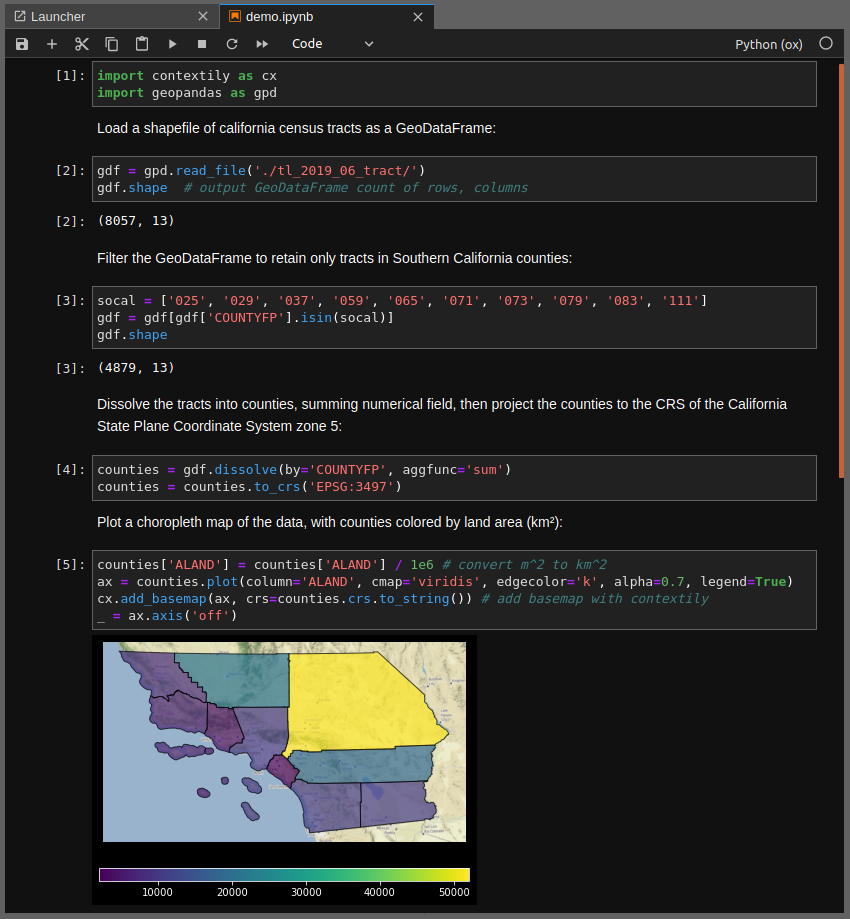
\includegraphics[width=0.8\textwidth]{code-demo.png}
	\caption{Simple real-world usage example that demonstrates basic GIS in a computational notebook, using JupyterLab and Python.}
	\label{fig:code_demo}
\end{figure*}

We conclude this chapter with a real-world usage example using JupyterLab and Python that demonstrates the absolute basics of doing GIS in a computational notebook, illustrated in Figure \ref{fig:code_demo}. In cell 1, we import the geopandas package for geospatial data handling and give it the friendly standard \enquote{gpd} handle. In cell 2, we use geopandas to read an ESRI shapefile containing all the census tracts in California, turn it into a GeoDataFrame, and output the shape of the resulting GeoDataFrame. We have 8,057 rows (i.e., census tracts) and 13 columns (i.e., variables). In cell 3, we create a list of all the county IDs in Southern California, then filter the GeoDataFrame to only retain tracts whose county IDs appear in that list. Outputting the shape of the resulting GeoDataFrame here reveals that we have retained only 4,879 of the original 8,057 tracts.

In cell 4, we dissolve and project the GeoDataFrame. First we aggregate the tracts up to the county level with a standard spatial dissolve operation and sum their numerical attributes to get new county totals. Then we project the GeoDataFrame from its original coordinate reference system (as defined in the shapefile) to a new one representing the meter-based California State Plane Coordinate System zone 5. Finally, in cell 5, we convert the land area column from m\textsuperscript{2} to km\textsuperscript{2}, then plot a (very basic) choropleth map of the spatial data, with counties colored by land area. This notebook can be executed linearly like a script by running it from the top-down, or it can be executed nonlinearly by a user choosing individual cells to run one or multiple times in an arbitrary order.

\setlength{\bibsep}{0.00cm plus 0.05cm}
\bibliographystyle{apalike}
\bibliography{GIS-BoK}

\section*{Learning Objectives}

TBD after first draft

\section*{Instructional Assessment Questions}

TBD after first draft

\section*{Additional Resources}

TBD after first draft

should include Dani's GDS course resources

\section*{Associated Image}

Figure \ref{fig:jupyterlab_interface} can be used as the associated image.

\end{document}
